\documentclass{article}

% ---------------------------------------------------------------------------------------------------------------
% Atlas-5K 10M. Build: pdflatex main && bibtex main && pdflatex main && pdflatex main
% Every number is copied from a run log or result file named in the text (Colab run w5k_atlas_10m_h24_g1 and
% w5k_atlas_1m_h24_v2c_final, Kaggle runs atlas-w5k-*); rules are in atlas/README.md, sections "Atlas-5K 10M" and
% "World benchmarks", committed to GitHub before the runs they govern.
% ---------------------------------------------------------------------------------------------------------------
\newif\ifpreprint
\preprinttrue
\ifpreprint
  \usepackage[preprint]{neurips_2025}
\else
  \usepackage{neurips_2025}
\fi
\makeatletter\renewcommand{\@noticestring}{Preprint.}\makeatother % not under review anywhere: replace the style's "Preprint. Under review."

\makeatletter
\renewcommand{\@neuripsordinal}{41st}
\renewcommand{\@neuripsyear}{2027}
\makeatother

\usepackage[utf8]{inputenc}
\usepackage{hyperref}
\usepackage{url}
\usepackage{booktabs}
\usepackage{amsfonts,amsmath,amssymb}
\usepackage{microtype}
\usepackage{xcolor}
\usepackage{graphicx}
\usepackage{caption}
\captionsetup{font=small,labelfont=bf}
\usepackage{enumitem}
\setlist{leftmargin=1.3em,itemsep=1pt,topsep=2pt}
\definecolor{atlasblue}{HTML}{1F5FBF}
\hypersetup{colorlinks=true,linkcolor=atlasblue!75!black,citecolor=atlasblue!75!black,urlcolor=atlasblue!75!black}

\title{Grow, Don't Restart: A 9.6M-Parameter Station World Model Grown from 1M Beats PhysicsFormer on WEATHER-5K at 24 Hours}

\ifpreprint
\author{%
  Aditya Kumar \qquad Anupam Singh\\
  ParadoxAI Lab\\
  \texttt{contact.paradoxailab@gmail.com}
}
\else
\author{Anonymous Author(s)\\Affiliation\\Address\\\texttt{email}}
\fi

\begin{document}
\maketitle

\begin{abstract}
We study whether a compact numerical world model for weather stations should be scaled by training a larger model from
scratch or by \emph{growing} a trained small one. Atlas-5K is a station-graph model: each station reads its last 48 hours
together with its 31 nearest neighbours, encodes them into a latent state, and rolls the state forward with one shared
transition network and geometry-biased attention between stations. Starting from our adopted 0.97M-parameter model, we
grow it to 9.64M parameters with an exact, function-preserving map (width doubled by tiling with zero-sum perturbations,
new blocks appended as the identity) and train it for 80,000 further steps. Under rules committed before the run, the
grown model was adopted on the 2022 validation year (standardised error $E=0.27592$, $-1.95\%$ against its parent) and
then scored once on the 2023 test year of the WEATHER-5K benchmark: all 5,672 stations, every hourly window,
$1.18\times10^9$ scored values per variable. At a 24-hour horizon its mean absolute error is lower than that of
PhysicsFormer (19.3M parameters), the benchmark's best published time-series model, on four of five variables
(temperature $-7.8\%$, dew point $-6.6\%$, wind direction $-6.0\%$, wind speed $-2.2\%$) with half the parameters,
and higher on sea-level pressure ($+3.3\%$). It also has lower error than the ECMWF-HRES operational forecast at the
stations on temperature, dew point, wind speed and wind direction, but much higher error on pressure ($+72\%$), so it
does not beat ECMWF-HRES under our pre-registered rule. The comparison with published models is by number only, since
their forecasts are not public. Ten-times larger models trained from scratch had failed to beat 1M on a far smaller
all-India data set; on WEATHER-5K growth paid, which is consistent with a size threshold that moves with data. The
whole run cost about 2.5 A100-hours. Code, rules, logs and the model file are public.
\end{abstract}

\section{Introduction}

Station forecasting --- predicting the next hours of temperature, humidity, wind and pressure at the places where
they are measured --- is where weather information is used. Global numerical weather prediction (NWP) models such as
ECMWF's operational high-resolution forecast (HRES) and AI weather models trained on reanalysis
\citep{lam2023graphcast,bi2023pangu} forecast gridded fields, which are then interpolated to stations. Time-series
models instead learn directly from station histories. WEATHER-5K \citep{han2026weather5k} puts both on one footing:
5,672 stations from NOAA's Integrated Surface Database \citep{smith2011isd}, hourly from 2014 to 2023, a fixed
train/validation/test split, and published scores for many time-series models from 0.0002M to 666M parameters, for
time-series foundation models, and for ECMWF-HRES at the stations.

Our earlier work built Atlas, a compact (at most 10M parameters) numerical world model for sensor networks, and found on
Indian air-quality stations that larger Atlas models trained from scratch did not beat a 1M-parameter one: there, the
data, not the size, set the error. WEATHER-5K holds about 40 times more
station-hours. This paper asks two questions: does size pay on data this large, and if so, is it better to restart at
the larger size or to grow the trained small model?

\paragraph{Contributions.}
\begin{itemize}
\item An exact growth map for Atlas (Section~\ref{sec:grow}): width $\times2$ and appended blocks, such that the grown
model computes the same forecasts as its parent at the start (largest difference $2.6\times10^{-5}$ on outputs of about
1.2), while duplicated units receive different gradients.
\item A pre-registered evaluation (Section~\ref{sec:protocol}): adoption rule on validation, a single test-year scoring,
and predictions written down before the run.
\item Results (Section~\ref{sec:results}): the grown 9.64M model has the lowest 24-hour error of any time-series model
reported on WEATHER-5K for four of five variables, beating PhysicsFormer by number with half its parameters; its
1M parent already does so on the same four variables. Pressure remains the gap to both PhysicsFormer and ECMWF-HRES.
\end{itemize}

\section{Related work}

\textbf{Station and time-series forecasting.} General forecasters such as DLinear \citep{zeng2023dlinear}, PatchTST
\citep{nie2023patchtst}, iTransformer \citep{liu2024itransformer} and Pyraformer \citep{liu2022pyraformer} model each
series (or each set of channels) without the stations' geometry; WEATHER-5K reports them with physics-informed variants,
of which PhysicsFormer is the strongest \citep{han2026weather5k}. Spatio-temporal graph models
\citep{li2018dcrnn,wu2019graphwavenet,shao2022stid} share information between sensors through a learned or fixed graph,
as Atlas does through attention biased by geometry. Time-series foundation models
\citep{das2024timesfm,ansari2024chronos,ansari2025chronos2} forecast zero-shot from a single series' history.

\textbf{Growing networks.} Function-preserving growth was introduced by Net2Net \citep{chen2016net2net} and extended to
transformers by bert2BERT \citep{chen2022bert2bert}, progressive stacking \citep{gong2019stacking} and learned growth
operators \citep{wang2023ligo}, mainly to save compute when training large language models. We use the same idea for a
different reason: to keep what a small model has learned about the stations while giving it more capacity, on a data
set large enough for the capacity to matter.

\textbf{Scaling.} Power laws in data and parameters \citep{kaplan2020scaling,hoffmann2022chinchilla} and transfer
\citep{hernandez2021scaling} describe when size pays. Our earlier threshold-function measurements on Indian stations
found the parameter term near zero at 1--10M parameters; the present result is a second point on that question.

\section{Atlas-5K}
\label{sec:model}

\textbf{Inputs.} For a station $s$ and a forecast start $t$, the model reads its 32-station neighbourhood (itself and
its 31 nearest stations on the sphere): for each, 48 hours of the five variables standardised by the benchmark's
scaler, a mask of observed values (missing values are not filled), and sine/cosine features of the hour of day and
day of year for the 48 input and 24 output hours. Static inputs are latitude, longitude and elevation; pair geometry is
the east and north offset and the distance between every two stations of the neighbourhood.

\textbf{Model.} A linear map embeds each station's window into a $d$-dimensional state; $n_e$ residual blocks
(LayerNorm, linear $d\to2d$, GELU, linear $2d\to d$) encode it; attention between the 32 stations, with a per-head bias
computed by a small MLP from the pair geometry, exchanges information. The latent dynamics then apply \emph{one} shared
transition six times, each step covering four forecast hours: the step's future time features are added to the state,
$n_d$ residual blocks and the same spatial attention update it, and a linear decoder reads that step's four hours. The
median forecast is each station's last observed value plus the decoded correction; the 10\% and 90\% quantiles are
the median minus and plus learned non-negative spreads, so they cannot cross. Training minimises the pinball loss
\citep{koenker1978quantile} on observed future values plus 0.2 times the absolute error of reconstructing 15\% of the
observed inputs, hidden at random; the median is scored.

\textbf{The parent: v2c.} $d=196$, 4 heads, $n_e=n_d=2$: 968,672 parameters. Trained on all 2014--2021 days of all
stations (16.6M station-days) for up to 150,000 steps with batches of 256 neighbourhoods (AdamW
\citep{loshchilov2019adamw}, one-cycle schedule \citep{smith2019onecycle}, peak learning rate $10^{-3}$), it stopped by
patience at 146,000 steps (best at 134,000). Its first version, v1 (16-station neighbourhoods, 60,000 steps), had
validation $E=0.29292$; v2c reached $E=0.28140$ ($-3.93\%$) and was adopted.

\section{Growing Atlas}
\label{sec:grow}

Let the residual stream of the parent have width $d$ and $h$ heads of size $d/h$. The grown model has width $fd$ and
$fh$ heads of the same size ($f=2$ here). Every stream vector is tiled, $z' = [z, z, \ldots, z]$. Because LayerNorm
\citep{ba2016layernorm} computes the mean and variance over the vector, $\mathrm{LN}(z') = [\mathrm{LN}(z),\ldots]$ when
its gain and bias are tiled too, so every layer can be mapped exactly:
\begin{itemize}
\item a linear layer that \emph{writes} the stream, or a hidden layer, has its output rows tiled;
\item a linear layer that \emph{reads} a tiled vector has its input columns tiled and divided by $f$, plus a
perturbation that sums to zero over the copies: copy $i$ gets $W/f + \varepsilon_i$ with $\sum_i \varepsilon_i = 0$
($\varepsilon$ Gaussian with 5\% of the weights' spread). Since the $f$ inputs are identical,
$\sum_i (W/f+\varepsilon_i)x = Wx$ exactly, yet the copies receive different gradients, so they can specialise. Plain
duplication (Net2Net's widening) would keep them identical forever;
\item attention: query, key and value projections are tiled per head (new head $j$ is old head $j \bmod h$); the
geometry bias MLP's output is tiled per head; the scale $1/\sqrt{d/h}$ is unchanged because the head size is;
\item depth: new encoder and transition blocks are appended with their output layer set to zero, so each starts as the
identity and still receives a gradient through its output layer.
\end{itemize}
With $f=2$, $n_e: 2\to7$ and $n_d: 2\to7$, v2c grows to $d=392$, 8 heads and \textbf{9,639,780} parameters, under the
10M cap. On random inputs the grown model's quantiles differ from v2c's by at most $2.6\times10^{-5}$ (mean output
magnitude about 1.2), and its validation error before any training was 0.2796, equal to v2c's on the same stations
(check G0, Section~\ref{sec:protocol}). The code is \texttt{atlas/grow.py}.

\textbf{Continued training.} As v2c except: peak learning rate $3\times10^{-4}$ (the start is already trained), 3\%
warm-up then one-cycle decay, weight decay $10^{-4}$, 80,000 steps, validation every 2,000 steps on 300 fixed stations,
best checkpoint kept. One NVIDIA A100-SXM4-80GB on Google Colab: 0.067\,s per step, 103.4 minutes.

\section{Protocol}
\label{sec:protocol}

\textbf{Benchmark.} WEATHER-5K's protocol, unchanged \citep{han2026weather5k}: 48 input hours; train 2014--2021,
validate 2022, test 2023; MAE per variable averaged over lead hours 1--24 in the variables' own units, over every hourly
window of every station. Our pipeline reproduces the benchmark's published DLinear scores within 3\% (temperature
3.469 against 3.57, averaged over the four lead times), which we required before scoring any Atlas model.

\textbf{Rules} (committed to the public repository before the run; README sections ``Atlas-5K 10M'' and ``World
benchmarks''):
\begin{enumerate}
\item \emph{Check G0}: the grown model's step-0 validation equals v2c's on the same 300 stations within 0.5\%.
\item \emph{Rule 10M-A}: $E$ = the mean over the five variables of validation MAE divided by the benchmark's scale
(every 4th station, every 6th hour of 2022). The grown model is adopted if $E \le 0.2786$, i.e.\ at least 1\% below
v2c's 0.28140. Only if adopted is it scored, once, on 2023; this was enforced in code (\texttt{--test-if-below}).
\item \emph{Rule WB1}: beating PhysicsFormer needs lower test MAE on at least four of five variables; beating ECMWF-HRES
needs lower MAE on temperature, dew point, wind speed and pressure. Comparisons with published numbers are by number
only: the published forecasts are not available for a paired test.
\end{enumerate}
\textbf{Predictions} (same commit): G0 passes (95\%); the grown model is adopted (60\%) with $E$ between 0.270 and 0.278
(60\%); v2c beats PhysicsFormer (60\%) and its pressure error stays higher (90\%); the grown model beats PhysicsFormer
(75\%) with its pressure error still above 1.43 (75\%); neither beats ECMWF-HRES (95\%).

\section{Results}
\label{sec:results}

\begin{figure}[t]
\centering
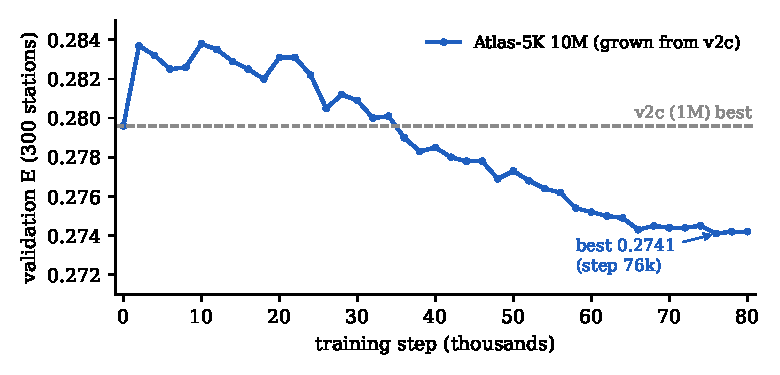
\includegraphics[width=0.78\linewidth]{figures/curve.pdf}
\caption{Validation error of the grown model on the 300 checking stations. Step 0 is the grown model before training,
equal to v2c's best (dashed). The error rises while the learning rate is high, falls below v2c at step 36,000, and
reaches 0.2741 at step 76,000 (kept).}
\label{fig:curve}
\end{figure}

\textbf{Training and adoption.} Check G0 passed (0.2796 against 0.2796). Figure~\ref{fig:curve} shows the validation
curve. Final validation on the rule's stations: MAE 1.418 / 1.482 / 53.86 / 1.188 / 1.484 (temperature, dew point, wind
direction, wind speed, pressure), $E = \mathbf{0.27592}$, $-1.95\%$ against v2c: \textbf{adopted}. Every variable
improved on v2c ($-3.1\%$, $-2.3\%$, $-1.6\%$, $-1.4\%$, $-3.4\%$).

\begin{table}[t]
\caption{WEATHER-5K, 2023 test, 24-hour horizon, MAE in the variables' units (\textdegree C, \textdegree C, degrees,
m/s, hPa). Atlas rows: all 5,672 stations, every hourly window, $1{,}182{,}816{,}192$ scored values per variable; each
model scored once. Published rows from \citet{han2026weather5k}.}
\label{tab:test}
\centering\small
\begin{tabular}{lrrrrrr}
\toprule
Model & Params & Temp. & Dew pt. & Wind dir. & Wind spd. & Pressure\\
\midrule
\textbf{Atlas-5K 10M (grown, ours)} & 9.64M & \textbf{1.429} & \textbf{1.486} & \textbf{53.93} & \textbf{1.183} & 1.477\\
Atlas-5K v2c (ours) & 0.97M & 1.474 & 1.520 & 54.84 & 1.202 & 1.533\\
Atlas-5K v1 (ours) & 0.97M & 1.553 & 1.596 & 56.46 & 1.228 & 1.664\\
\midrule
PhysicsFormer, published & 19.3M & 1.55 & 1.59 & 57.37 & 1.21 & 1.43\\
ECMWF-HRES at stations, published & -- & 1.76 & 1.85 & 63.8 & 1.48 & \textbf{0.86}\\
DLinear, our run & 0.002M & 2.659 & 2.438 & 66.64 & 1.439 & 3.107\\
Persistence, our run & -- & 3.743 & 2.229 & 75.48 & 1.747 & 2.735\\
\bottomrule
\end{tabular}
\end{table}

\begin{figure}[t]
\centering
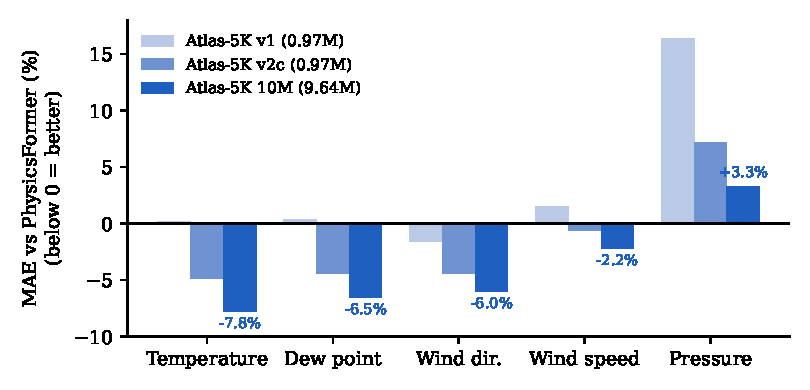
\includegraphics[width=0.8\linewidth]{figures/vs_physicsformer.pdf}
\caption{2023 test MAE relative to PhysicsFormer (19.3M), per variable. Below zero is better. Labels: the grown model.}
\label{fig:vspf}
\end{figure}

\textbf{Test year.} Table~\ref{tab:test} and Figure~\ref{fig:vspf}. Against PhysicsFormer the grown model is lower on
temperature ($-7.8\%$), dew point ($-6.6\%$), wind direction ($-6.0\%$) and wind speed ($-2.2\%$) and higher on
pressure ($+3.3\%$): it \textbf{beats PhysicsFormer} under rule WB1, with half its parameters. Its parent v2c also beats
it under the same rule ($-4.9\%$, $-4.4\%$, $-4.4\%$, $-0.7\%$; pressure $+7.2\%$) with a twentieth of the parameters;
the earlier v1 did not (one of five). Against ECMWF-HRES the grown model is lower on temperature ($-18.8\%$), dew point
($-19.7\%$), wind speed ($-20.1\%$) and wind direction ($-15.5\%$) but far higher on pressure ($+72\%$): \textbf{it does
not beat ECMWF-HRES} under the four-variable rule. Test MSE: 5.023 / 5.782 / 6798.3 / 3.276 / 6.111. Validation and test
agree within 1\% for both v2c and the grown model. All eight predictions held.

\textbf{Growth against restart.} On the all-India air-quality league, a 10M Atlas trained from scratch with weather
inputs was 1.0\% \emph{worse} than 1M at all data (validation MAE 8.773 against 8.684). On WEATHER-5K, the WB1-T data
curve of the 1M model flattens (validation $E$ 0.3376, 0.3129, 0.2971, 0.2929 at 1/64, 1/16, 1/4 and all of the
training days), which indicates the 1M model, not the data, was the limit; growing it to 10M then gained 1.95\% on
validation and 1.5--3.6\% per variable on test. We did not train a 10M model from scratch on WEATHER-5K in this study, so
we cannot say how much of the gain is due to growth rather than size; that comparison is part of the threshold grid in
progress (Section~\ref{sec:limits}).

\textbf{Cost.} About 2.5 A100-hours in total: training 1.7 hours, the remainder for the final validation and the
two single test scorings (the grown model and v2c).

\section{Limitations and next steps}
\label{sec:limits}
\begin{itemize}
\item \textbf{By number only.} PhysicsFormer's and ECMWF-HRES's forecasts are not public, so no paired significance
test against them is possible. Differences of 2--8\% on $1.18\times10^9$ values per variable are unlikely to be noise,
but published and our scores come from different code paths (ours reproduces DLinear within 3\%).
\item \textbf{One horizon.} Only 24 hours is reported. The benchmark also scores 72, 120 and 168 hours, where
PhysicsFormer and ECMWF-HRES are reported per lead; the other published models are reported only as averages over the
four leads, so we do not rank Atlas against them here.
\item \textbf{Pressure.} Sea-level pressure is the one variable where both PhysicsFormer and ECMWF-HRES are better. A
48-hour station history carries little of the synoptic-scale pressure change that a global model represents; longer
histories and wider neighbourhoods are the next tests.
\item \textbf{Growth vs restart.} Not isolated (above).
\item \textbf{In progress, pre-registered:} a paired head-to-head with TimesFM 2.5 and 3.0, Chronos-2 and Chronos-Bolt
on identical windows, and a size $\times$ data grid (0.1M--10M $\times$ 1/64--all of the data) to fit and verify the
threshold function $E(N,P)$ of Atlas on WEATHER-5K.
\end{itemize}

\section{Reproducibility}
\begin{itemize}
\item Repository: \url{https://github.com/paradoxailab/paradox-world-model}, branch \texttt{atlas-v0.1}.
\item Model \texttt{atlas/atlas/model.py}; growth \texttt{atlas/atlas/grow.py}; training and scoring
\texttt{atlas/delhi/run\_atlas\_5k.py}; Colab notebook \texttt{atlas/notebooks/atlas\_10m\_colab.ipynb}.
\item Rules, predictions and results: \texttt{atlas/README.md} (committed before each run).
\end{itemize}
The run command:
\begin{quote}\small\texttt{python run\_atlas\_5k.py --init 57\_atlas-5k\_v2c\_weather5k\_adopted.pt --grow 2,7,7 --k 32
--steps 80000 --lr 3e-4 --no-test --test-if-below 0.2786}\end{quote}
Model files hold their dataset name, configuration and results: v2c is \texttt{models/series/57\_\ldots}; the grown
model is released as \texttt{models/series/58\_atlas-5k-10m\_weather5k\_adopted.pt}.

\bibliographystyle{plainnat}
\bibliography{refs}

\end{document}
